
\chapter{Genome Graphs}
\label{ch:bakeoff}

This chapter has been adapted from the article \citet{novak2017genome}, and contains material attributable to all authors of that work. Supplementary materials referenced here are available in the online version of that article.

\section{Abstract}

There is increasing recognition that a single, monoploid reference
genome is a poor universal reference structure for human genetics,
because it represents only a tiny fraction of human variation. Adding
this missing variation results in a structure that can be described as a
mathematical graph: a genome graph. We demonstrate that, in comparison
to the existing reference genome (GRCh38), genome graphs can
substantially improve the fractions of reads that map uniquely and
perfectly. Furthermore, we show that this fundamental simplification of
read mapping transforms the variant calling problem from one in which
many non-reference variants must be discovered de-novo to one in which
the vast majority of variants are simply re-identified within the graph.
Using standard benchmarks as well as a novel reference-free evaluation,
we show that a simplistic variant calling procedure on a genome graph
can already call variants at least as well as, and in many cases better
than, a state-of-the-art method on the linear human reference genome. We
anticipate that graph-based references will supplant linear references
in humans and in other applications where cohorts of sequenced
individuals are available.

\section{Introduction}

The human reference genome, completed in draft form in 2001 and revised
several times subsequently \cite{Lander2001-gm,Church2011-ob}, is the
single most important resource used in human genetics today. It acts as
a universal coordinate system and as such is the space in which
annotations (genes, promoters, etc.) and genetic variants are described
\cite{Harrow2012-ei,ENCODE_Project_Consortium2012-rx,1000_Genomes_Project_Consortium2015-mp}.
It is also the target for read mapping, and, downstream of this mapping,
is used for functional assays and variant calling pipelines
\cite{Li2009-tj,depristo2011framework}.

The contemporary definition of a reference genome is completely linear:
a single monoploid assembly of the genome of a species. A key limitation
of the linear human reference genome (the set of chromosome scaffolds)
is that it is but a single genome. As such, it is an imperfect lens
through which to study our population's variation; there exist variants
and annotations that can not be easily described with respect to the
reference genome \cite{horton2008variation,Pei2012-xo}. Furthermore, as a
target for mapping and interpretation it introduces a reference allele
bias: a tendency to over-report alleles present in the reference genome
and under-report other alleles \cite{degner2009effect,brandt2015mapping}. To
mitigate these issues, recent versions of the reference genome assembly,
such as GRCh38, have contained ``alternate locus'' sequences (``alts''):
extra sequence representations of regions of the human genome considered
to be highly polymorphic, anchored at their ends to locations within the
``primary'' (monoploid) reference assembly. Such a structure, which
contains multiple partially-overlapping sequence paths, can be
considered a form of mathematical graph. The explicit use of graphs in
biological sequence analysis has a long history, notably for sequence
alignment \cite{Paten2014-ga}, sequence assembly
\cite{Pevzner2001-lm,Myers2005-oi}, assembly representation (as in FASTG
and now GFA)\cite{fastg2016fastg,GFA-spec_contributors_undated-tg},
substring indexes (which are often thought of in terms of suffix trees
or similar data structures) \cite{Li2009-tj,Simpson2010-of}, and
transcript splice graphs \cite{Heber2002-pw}. Recently the notion of
graphs for representing genomes has been considered explicitly
\cite{dilthey2015improved,Paten2014-ga,maciuca2016natural}, and work has been
done towards using these graphs as references \cite{Limasset2016-by}.
The alternate loci currently used are just one way to extend the linear
reference genome into a genome graph; many other ways are possible. In
this work, conducted by a task team of the Global Alliance for Genomics
and Health, we experiment with different methods for graph construction
and testing the utility of different graphs for read mapping and variant
calling. This work is the first study of its kind that we are aware of.
We attempt to test the simple hypothesis that adding data into the
reference structure---in effect, adding to the ``reference prior'' on
variation extant in the population---will result in improved genome
inferences.

\section{Results}

There are many possible types of genome graph; here we use
\emph{sequence graphs}. The nodes of a sequence graph are a set of DNA
sequences. Each node is therefore a string of nucleotide characters,
called positions, giving the sequence of the node's forward strand. We
call the terminal 5' and 3' ends of this strand the \emph{sides} of the
node. Each edge in the graph is an unordered pair of sides, representing
a (potential) bond between two sides of a pair of nodes. This is a
bidirected graph representation, because features of the edge indicate
to which side of a node (sequence), 5' or 3', each end of the edge
connects (Fig. \ref{fig:bakeoff:example})\cite{Medvedev2009-hy}. Other representations of genome
graphs, such as the directed acyclic representation, can be useful; see
Supplementary Section 1. A longer DNA sequence can be represented as a
\emph{thread} within a sequence graph, beginning in one oriented node,
ending in the same node or another, and in between walking from node to
node, with the rule that if the walk enters a node on one side it exits
through the other side.

\begin{figure}[htbp]
\centering
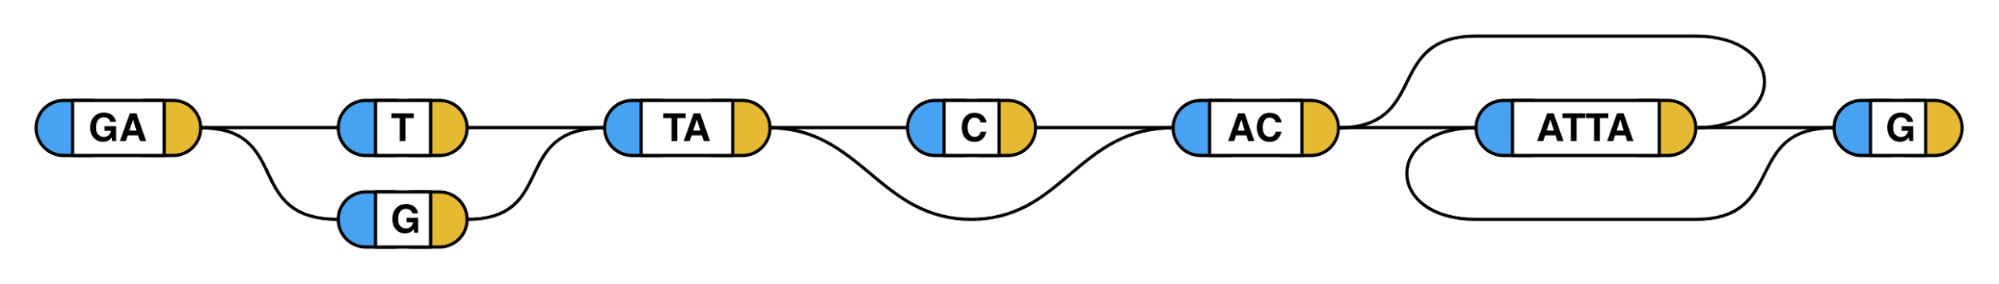
\includegraphics[width=\textwidth]{figures/04_bakeoff/figure01.png}
\caption[Example sequence graphs]{Example sequence graphs. Each node holds a string of bases. An
edge can connect, at each of its ends, to a base on either the left (5',
blue) or the right (3', yellow) side of the node. When reading through a
thread to form a DNA sequence, a valid walk must leave each node via the
opposite side from that through which it was entered; a node's sequence
is read as reverse-complemented if the node is entered on the 3' side.
One thread that this graph spells out (reading from the left side of the
leftmost sequence to the right side of the rightmost sequence, along the
nodes drawn in the middle) is the sequence ``GATTACACATTAG''. Straying
from this path, there are three variants available: a substitution of
``G'' for ``T'', a deletion of a ``C'', and an inversion of ``ATTA''. If
all of these detours are taken, the sequence produced is
``GAGTAACTAATG''. All 8 possible threads from the leading G to the
trailing G are allowed.}
\label{fig:bakeoff:example}
\end{figure}



To evaluate the utility of sequence graphs we invited teams to construct
and evaluate graphs for five test regions of the human genome: the major
histocompatibility complex (MHC), the killer cell immunoglobulin-like
receptors (LRC\_KIR) region, the spinal muscular atrophy (SMA) locus,
and the BRCA1 and BRCA2 genes. MHC, SMA and LRC\_KIR are all regions
with alternate loci represented in GRCh38, while BRCA1 and BRCA2
represent more typical human genes. Regions ranged from 81 kilobases in
size with a single gene (BRCA1) to 5.0 megabases in size with 172 genes
(MHC). We considered graphs from five teams built with eight different
pipelines (Table \ref{tbl:bakeoff:graphs}). For each region we provided a set of long, high
quality input sequences from which to construct graphs (Table \ref{tbl:bakeoff:regions}), but
also encouraged the creation of graphs using additional data of the
builder's choice. Some graphs were built based upon existing variant
calls, such as the 1000 Genomes calls used to construct the 1KG graph
\cite{1000_Genomes_Project_Consortium2015-mp}. Graphs were also built
with a wide variety of different algorithmic approaches (Table \ref{tbl:bakeoff:graphs}). Three
control graphs were constructed for each region as points of comparison.
The Primary graphs contain just the single, linear reference path from
GRCh38. The Unmerged graphs consist of just the set of provided
sequences, each represented as a disjoint path. The Scrambled graphs
(see Online Methods) are essentially identical topologically to the 1KG
graphs, but with structures shifted to create false variants. These
graphs acted as a negative control for the effects of adding nonsense
variation to the graphs.

\begin{table}
  \centering
  {\small
  \begin{tabular}{lp{1.5cm}p{1.5cm}p{2cm}p{1.5cm}p{1.5cm}}
  \textbf{Region} & \textbf{Chromo\-some} & \textbf{Length in Primary Reference (bp)} & \textbf{GRCh38 Coordinates} & \textbf{Number of Genes} & \textbf{Alt Haplotypes in pilot data}
  \\
  \hline
  BRCA1 & 17 & 81,189 & 43044293-43125482 & 1 & 2
  \\
  BRCA2 & 13 & 84,989 & 32314860-32399849 & 1 & 2
  \\
  LRC\_KIR & 19 & 1,058,685 & 54025633-55084318 & 47 & 35
  \\
  MHC & 6 & 4,970,458 & 28510119-33480577 & 172 & 8
  \\
  SMA & 5 & 2,397,625 & 69216818-71614443 & 21 & 2
  \end{tabular}
  }

  \caption[Pilot regions]{Pilot Regions. Selected test cases represent
a sampling of both typical and challenging genomic regions.}
  \label{tbl:bakeoff:regions}
\end{table}

\begin{FPtable}
  \centering
  {\small
  \begin{tabular}{p{2cm}p{1.5cm}p{1.5cm}p{5cm}}
  \hline
  \multicolumn{4}{c}{\textbf{Submissions using pilot data}}
  \\
  \hline
  \textbf{Submission} & \textbf{Team} & \textbf{Short Name} & \textbf{Description of Algorithm}
  \\
  \hline
  Cactus & UCSC & Cactus & Graph-based multiple sequence aligner \cite{paten2011cactus2}.
  \\
  Camel & UCSC & Camel & Creates graphs progressively by mapping using
  context schemes \cite{novak2015canonical}.
  \\
  De Bruijn Graph (k=63) & MSKCC & De Bruijn 63 & Forms a De Bruijn graph
  of input data with k=63, then converts to a sequence graph.
  \\
  Population Reference Graph & Oxford & PRG & Creates a graph from a
  K-mer-based HMM description of a region \cite{dilthey2015improved}.
  \\
  Seven Bridges & Seven Bridges & 7BG & Multiple genome alignment.
  \\
  \hline
  \multicolumn{4}{c}{\textbf{Submissions using other data}}
  \\
  \hline
  \textbf{Submission} & \textbf{Team} & \textbf{Short Name} & \textbf{Description of Algorithm}
  \\
  \hline
  1000 Genomes SNP Graph & Sanger/\allowbreak UCSC & 1KG & Generated using vg
  construct on a VCF containing variants identified in the 1000 genomes
  project. Platinum genome samples were not included, to avoid circularity
  in variant evaluation.
  \\
  1000 Genomes Haplotype 50 & Sanger/\allowbreak UCSC & 1KG Haplo 50 & Adapted form of
  1KG graph in which phasing information is used to reduce the number of
  unobserved recombinations represented by the graph. 50~is the number of
  bases two variants can be apart to be considered for this phasing.
  \\
  Scrambled 1000 Genomes & Sanger/\allowbreak UCSC & Scrambled & Generated by shifting
  all the variants in the standard 1KG graph 200~bp downstream.
  \end{tabular}
  }

  \caption[Genome graph submissions]{Genome Graph Submissions. Submissions were collected from a variety of institutions, and showcase a variety of graph construction methods.}
  \label{tbl:bakeoff:graphs}
\end{FPtable}

\begin{FPfigure}
\centering
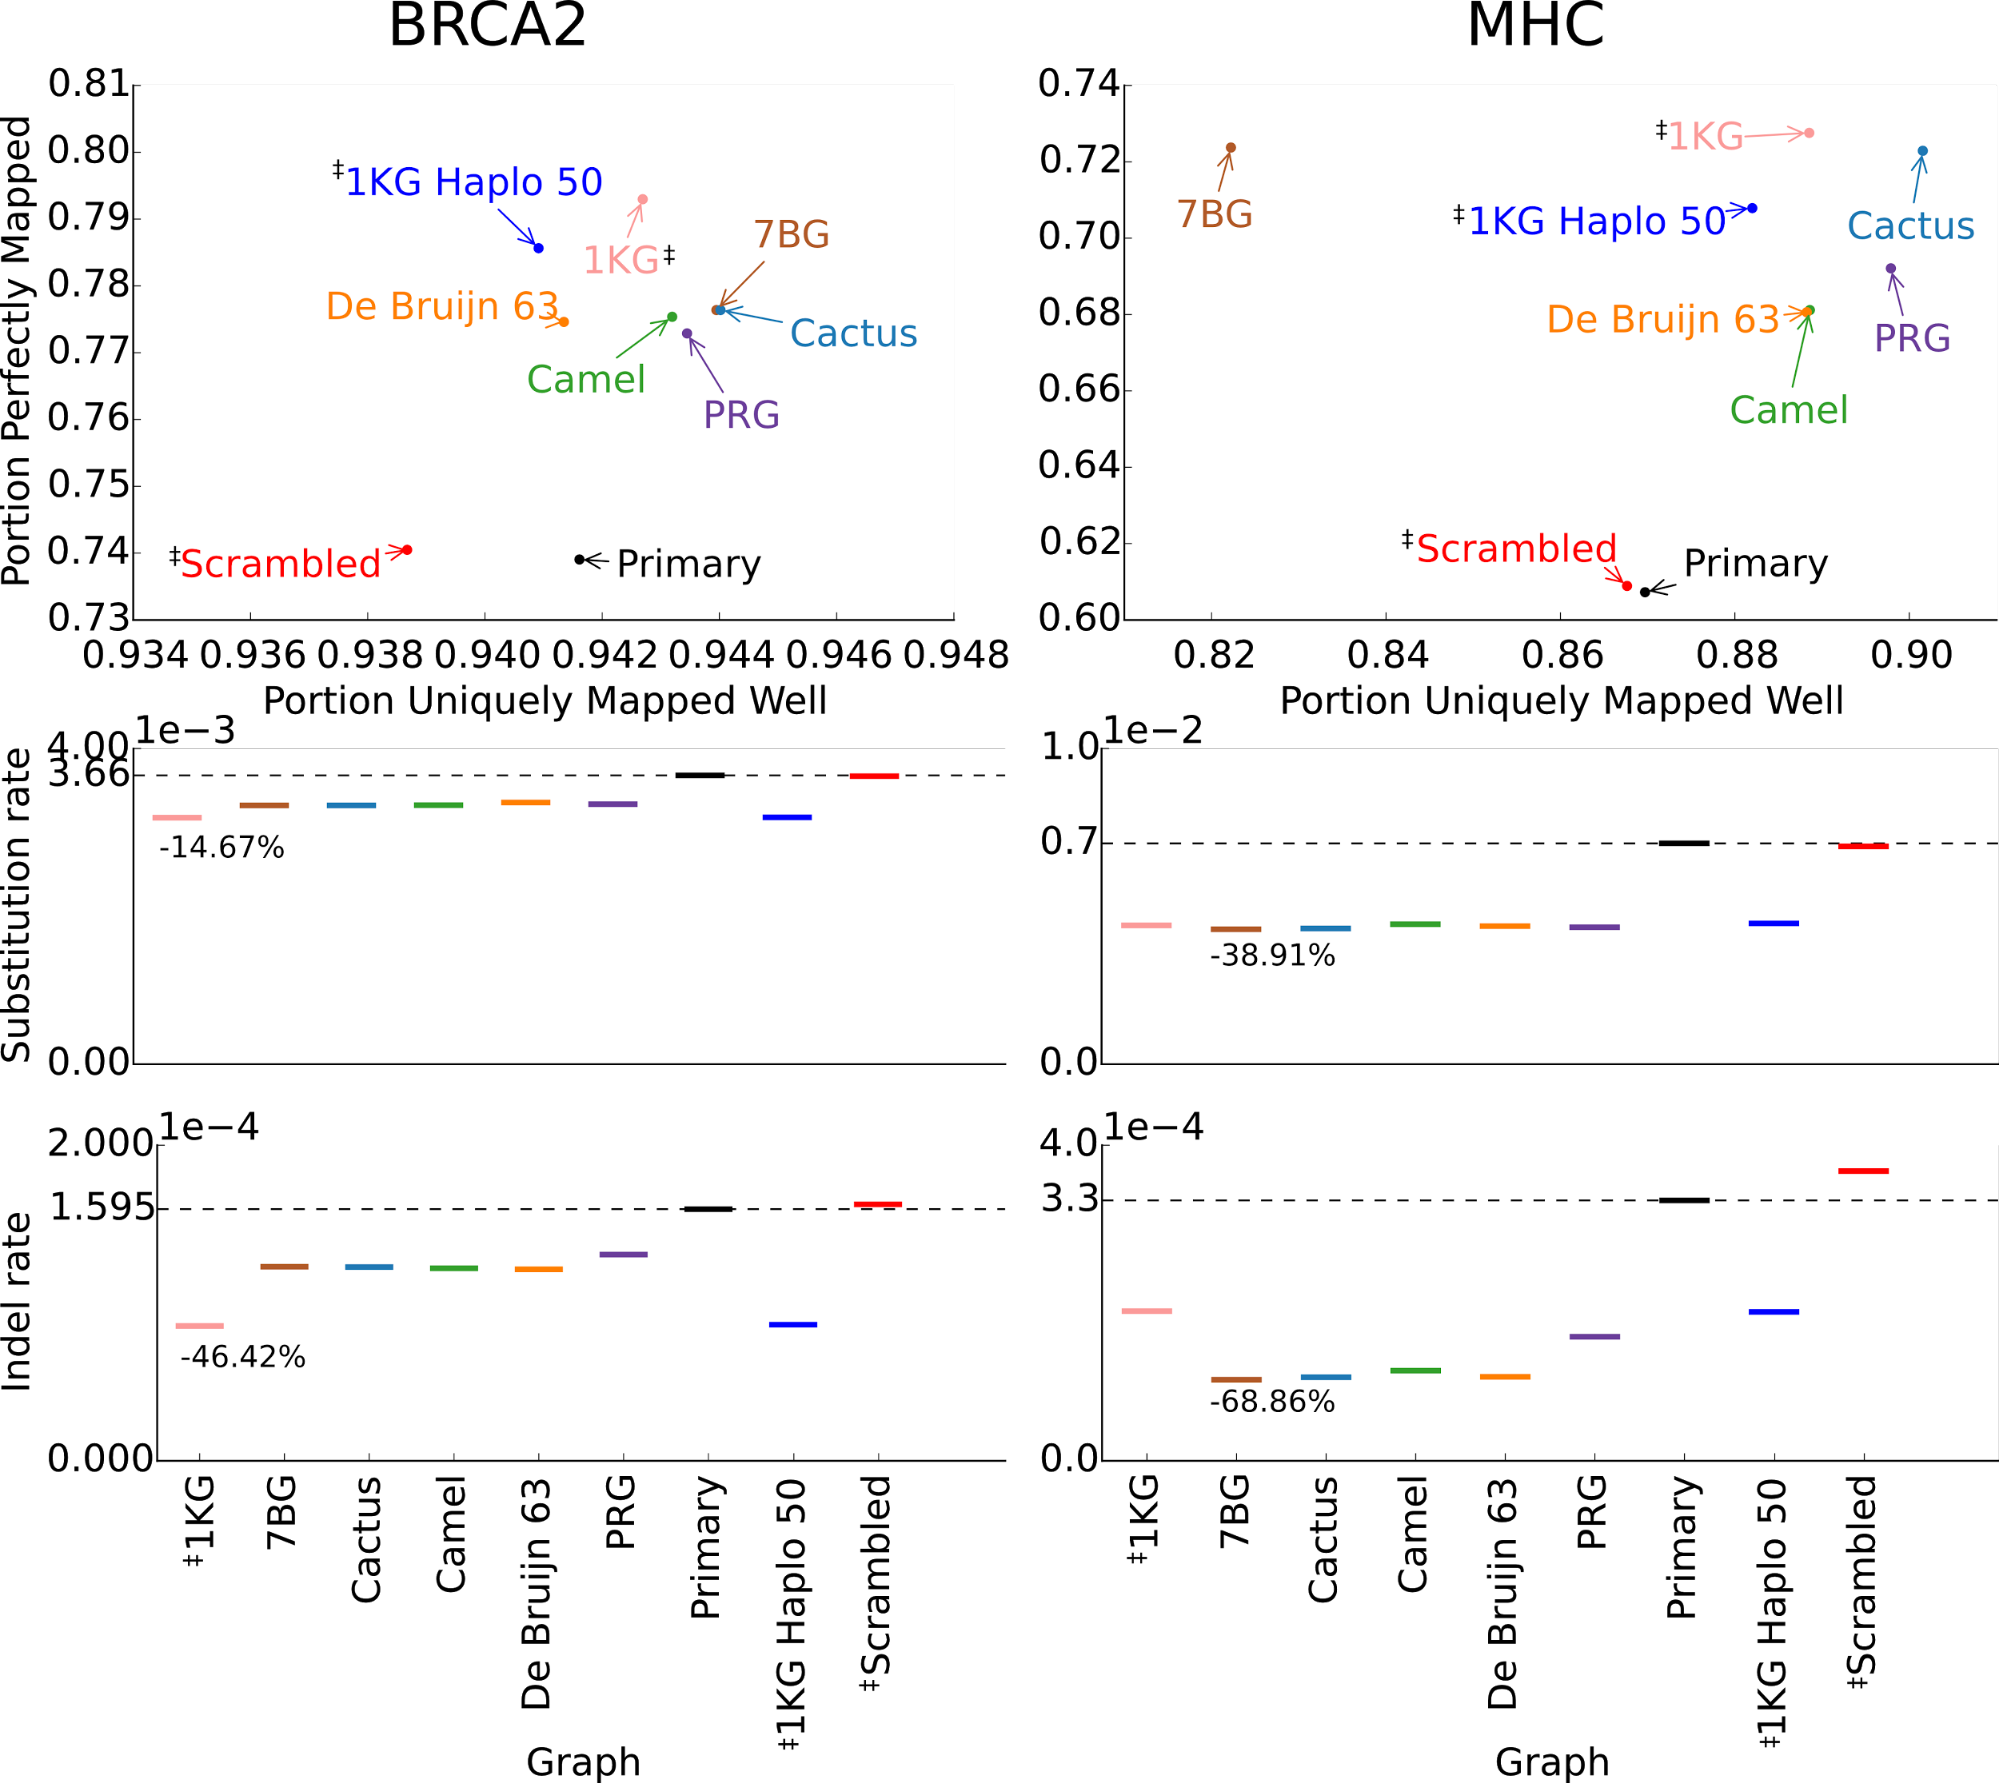
\includegraphics[width=\textwidth]{figures/04_bakeoff/figure02.png}
\caption[Mapping reads to sequence graphs]{Mapping reads to sequence graphs. Results for the 1000 Genomes
Phase 3 low coverage samples against the BRCA2 and MHC graphs. The
median per-sample portion of reads that are mapped perfectly (Y axis),
and the median per-sample portion of reads that are mapped with a
unique, obviously-best alignment (X axis) are both visible in the top
row. The median per-sample substitution rate for a primary mapping,
computed per aligned base, is shown in the second row. The median per
sample frequency of indels in primary mapped reads, computed per read
base, is given in the third row. The horizontal black line represents
the result for the primary reference graph in the region. The ‡ symbol
marks graphs generated using additional data beyond the provided
reference and alternate sequences. The unmerged graphs are excluded
because very few reads mapped uniquely to them.}
\label{fig:bakeoff:mapping}
\end{FPfigure}

\subsection{Graph Read Mapping}

To evaluate the utility of sequence graphs for read mapping we used the
software program vg\cite{Vgteam_undated-xe}, which contains a mapping
algorithm capable of mapping to a fully general and potentially cyclic
sequence graph (see Supplementary Section 2). We mapped all relevant
reads (see Online Methods) from 1000 Genomes Phase 3 low coverage
samples to each graph. We found that vg was able to map almost all such
reads to the graphs (Supplementary Fig. 3).

Relative to the primary graph, a graph containing more of the variants
should produce an increase in the fraction of reads that map perfectly
(without either substitutions or indels) to at least one place. For
BRCA2 we see a relative increase of 7.3\% in the median number of reads
mapping perfectly to the 1KG graph vs.~the Primary graph, but for MHC
the increase is 20\% (Fig. \ref{fig:bakeoff:mapping} top row, Supplementary Section 3,
Supplementary Fig. 1). The increase for BRCA2 is close to what would be
expected if the sequence graph contained the majority of polymorphisms
for a typical region of the genome (Supplementary Section 3), while the
larger increase for MHC is likely due to a greater degree of
polymorphism \cite{brandt2015mapping}. Similar, slightly smaller increases
are seen for graphs built from other, smaller collections of variants.
The scrambled graphs do not show significant gains, thus indicating that
the effect is specific to graphs containing known variation.
Furthermore, the overall substitution rate between reads and the
experimental graphs was observed to decrease, relative to the rate
between the reads and the Primary control graph. In the
highest-performing graphs the decline is slightly below the bounds of
previous read substitution error rate estimates of 0.7-1.6\%
\cite{Minoche2011-il,1000_Genomes_Project_Consortium2010-ky,1000_Genomes_Project_Consortium2012-gr,1000_Genomes_Project_Consortium2015-mp}
(Fig. \ref{fig:bakeoff:mapping} second row; see Supplementary Section 4 and Supplementary Fig.
4). The decrease in indel rate (Fig. \ref{fig:bakeoff:mapping} third row) moving from the
Primary graph to the 1KG graph is comparable to estimates of the human
indel polymorphism rate\cite{Mills2011-lj} (Supplementary Section 5).

The median fraction of reads that uniquely map increases for many of the
graphs, relative to the primary and scrambled graphs. For example, in
the Cactus graph, an increase of 0.26\% is observed in BRCA2, and an
increase of 3.7\% is observed in the MHC. No such increase in unique
mapping is seen for the comparably complex scrambled graph. Unique
mapping is defined as having a good primary mapping and no reasonable
secondary mapping (see Supplementary Section 3 and Supplementary Fig.
2).

To test if the choice of sequence graph reference affected population
level reference allele bias, we binned samples by 1KG super-population
and looked at the difference in perfect mapping between the 1KG graph
and the Primary graph for each subpopulation. We find a small but
significant difference in perfect mapping increase between
super-populations for most regions (Supplementary Section 6,
Supplementary Fig. 5), but we also find relatively large differences in
absolute rates of perfect mapping (Supplementary Fig. 6). These latter
differences suggest that super-population may be confounded with
sequencing batch, making drawing conclusions from this analysis quite
difficult.

\subsection{Graph Variant Calling}

We implemented a comprehensive, albeit basic, variant calling pipeline
based on the Samtools pileup approach \cite{Li2009-je}, modified to work
with sequence graphs (see Online Methods for more details). In summary
(Fig. \ref{fig:bakeoff:calling}), reads are mapped to the reference graph or \emph{base graph}
and a pileup is computed at each graph position and edge. An
\emph{augmented} \emph{graph} is created by extending the base graph
with additional sequences and edges representing possible variants
determined from the pileups. This graph is then analyzed for
\emph{ultrabubbles} (acyclic, tip-free subgraphs connected to the rest
of the graph by at most 2 nodes) which are treated as sites for
genotyping\cite{paten2017superbubbles}. Finally, thresholding heuristics
are used to emit a set of genotypes with sufficient read support, one
for each site, expressed in the coordinates of the GRCh38 primary
reference path as embedded in the graph (see Online Methods).

\begin{FPfigure}
\centering
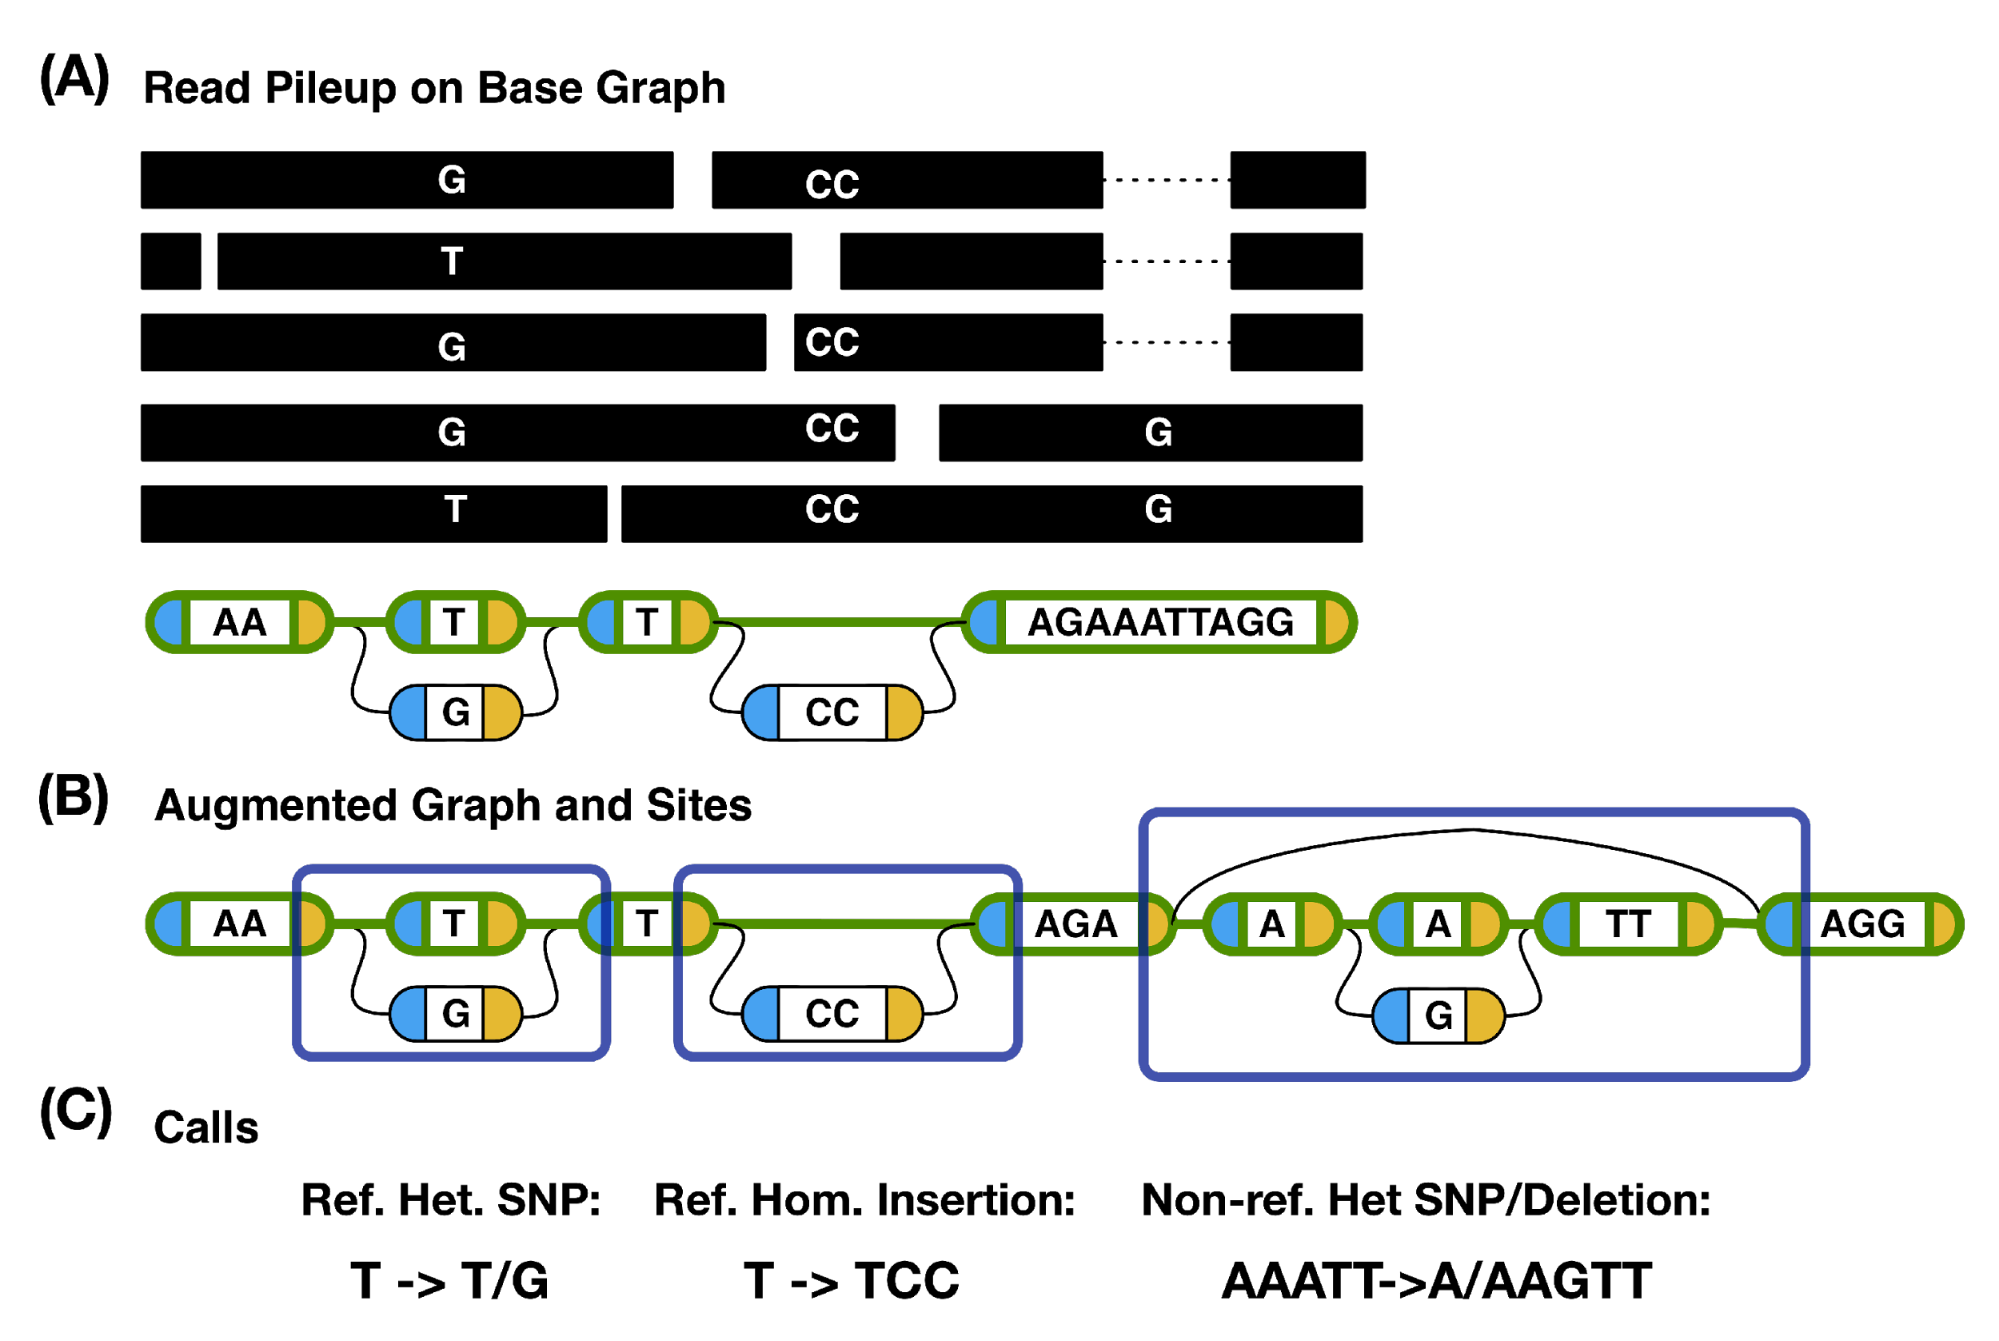
\includegraphics[width=\textwidth]{figures/04_bakeoff/figure03.png}
\caption[Variant calling with genome graphs]{Variant Calling with Genome Graphs. (A) Read pileup on a base
graph whose reference path is highlighted in green. Only variant or
non-reference base values are shown in the reads. (B) The augmented
graph contains the base graph as well as new structures implied by the
pileup. This graph contains three top-level ultrabubbles, each forming a
site. (C) Variant calls for each site. The first two (a heterozygous SNP
and a homozygous insertion) are considered reference calls because they
were present in the base graph, whereas the third (a heterozygous
combination of a SNP and a deletion) is non-reference because it was
novel to the augmented graph.}
\label{fig:bakeoff:calling}
\end{FPfigure}

We compared the results from the graph variant calling pipeline with the
Platinum Genomes benchmark data for samples NA12877 and
NA12878\cite{Eberle2016-zc} using vcfeval, which corrects for VCF
representation ambiguity by comparing at the haplotype level
\cite{Cleary2015-oy} \cite{Zook2014-tl}. To provide additional controls,
Freebayes \cite{garrison2012haplotype}, Platypus \cite{Rimmer2014-zj} and
Samtools \cite{Li2009-je} were run on BWA-MEM \cite{Li2009-tj}
alignments of the same input data to GRCh38 with their default options
in order to produce positive control variant calls. Figure \ref{fig:bakeoff:callingeval} (A) shows
the precision and recall of each method aggregated across both samples
and all regions. Figure \ref{fig:bakeoff:callingeval} (C) and (D) show precision-recall curves for
SNPs and indels, respectively. In comparison to the primary graph (the
graph containing only the existing reference sequence, and therefore a
control for the same variant calling algorithm applied to just the
knowledge in the existing reference), the 1KG and Cactus graphs'
F1-scores (Supplementary Table 1) increased by 3.50\% and 1.98\%,
respectively, increasing for both single nucleotide variants (3.13\%,
1.95\% respectively) and indels (6.02\%, 4.40\% respectively).
Furthermore, 1KG graphs have the overall highest accuracy (F1 score) of
all methods, although Samtools and Platypus perform best overall for
SNPs and indels, respectively. Supplementary Section 7 contains
additional breakdowns of the F1-scores by region (Supplementary Figs.
7-8), sample (Supplementary Fig. 9), and type (Supplementary Fig. 10),
as well as scores without clipping to confident regions (Supplementary
Fig. 11). Generally (in 13 out of 18 cases), the 1KG graph has higher
accuracy than both the primary and scrambled controls.

We define a \emph{reference} \emph{call} as a call asserting the
presence of a position or edge in the base graph. The experimental
graphs can dramatically reduce the number of non-reference calls, as
compared to control. For example, the Cactus and 1KG graphs reduce
non-reference calls by more than a factor of ten (Fig. \ref{fig:bakeoff:refnonref} (A)) relative
to the Primary reference graph. Furthermore, the precision of these
reference calls is higher than the non-reference calls for the
non-scrambled graphs (Fig. \ref{fig:bakeoff:refnonref} (B)).

Larger structural variants can be called using the same logic as point
mutations, provided they are already in the graph; Figure \ref{fig:bakeoff:refnonref} (C) displays
the indel length distribution for the two top-performing graphs and the
primary control, as well as a breakdown of indel lengths for reference
and non-reference calls. The reference call indel lengths in the
experimental graphs are larger than the Primary and non-reference
lengths and, in the case of Cactus, contain indels exceeding the read
length. This adds up to a large number of additional called bases: for
example, across the regions the Cactus graphs call 94 indel events
larger than 50 base pairs totaling 10045 bases, none of which are found
using the Primary graph with the same algorithm.

To mitigate potential biases with the Platinum Genomes benchmark data as
a truth set\cite{Eberle2016-zc}, we conducted what we term a
``reference-free'' evaluation of vg's variant calling accuracy, by
comparing against de novo assemblies instead of assumed-true variant
calls. In brief, short reads pooled from two haploid assemblies were
used to call variants on each sequence graph. The accuracy of this
reconstruction was evaluated using PacBio-based \emph{de novo} assembly
fragments, which by definition are free of reference artifacts and are
derived from a different sequencing technology (see Online Methods,
Supplementary Section 8 and Supplementary Figure 12). The results can be
seen in Figure \ref{fig:bakeoff:callingeval} (B) and Supplementary Figure 13. Several experimental
graphs have greater precision and recall than the Scrambled and Primary
controls; combined across all regions except SMA (which was
insufficiently covered by PacBio assemblies to be usefully analyzed), vg
on the Cactus graph outperformed existing methods. The results appear to
agree closely with those from the VCF-comparison-based evaluation,
considering that the two techniques use different sources of truth and
different evaluation metrics.

\begin{FPfigure}
\centering
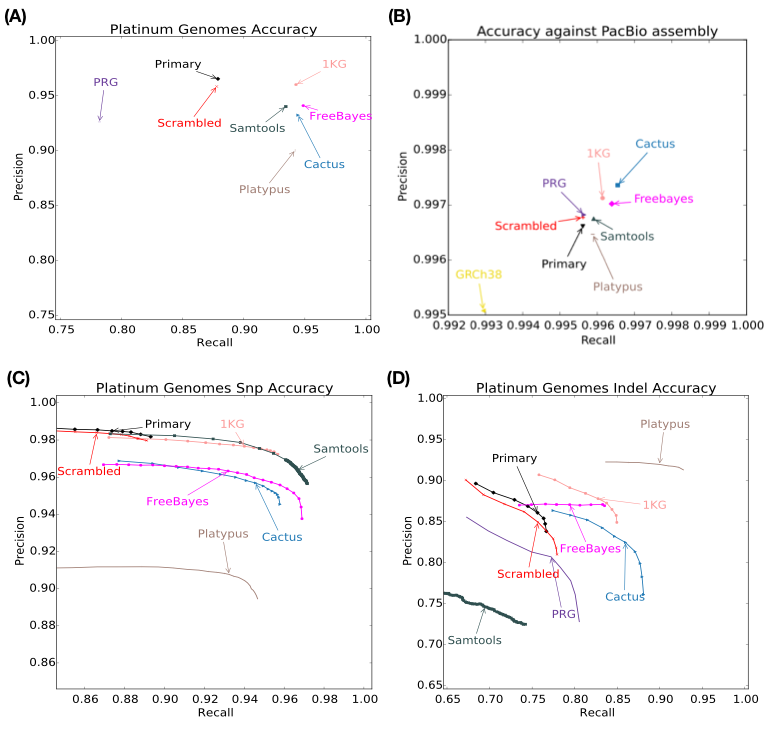
\includegraphics[width=\textwidth]{figures/04_bakeoff/figure04.png}
\caption[Variant calling evaluation]{Variant Calling Evaluation. (A) Precision (portion of called
variation in agreement with the truth set) and recall (portion of
variation in the truth set in agreement with what was called) against
the Platinum Genomes truth VCFs aggregated across NA12877 and NA12878
for all regions, as measured by vcfeval. (B) Per-base precision and
recall as measured by the reference-free evaluation in BRCA1, BRCA2,
LRC\_KIR, and MHC. The GRCh38 point shows a comparison of the existing
primary reference haplotype sequence against the de novo assembly. (C) -
(D) Breakdown of precision and recall from (A) into SNPs and indels,
respectively. Curves are shown by including accuracies at quality
thresholds that fall within a radius of 0.1 around the maximum F1. Full
results featuring F1-scores for all graphs are in Supplementary Section
7.}
\label{fig:bakeoff:callingeval}
\end{FPfigure}

\begin{FPfigure}
\centering
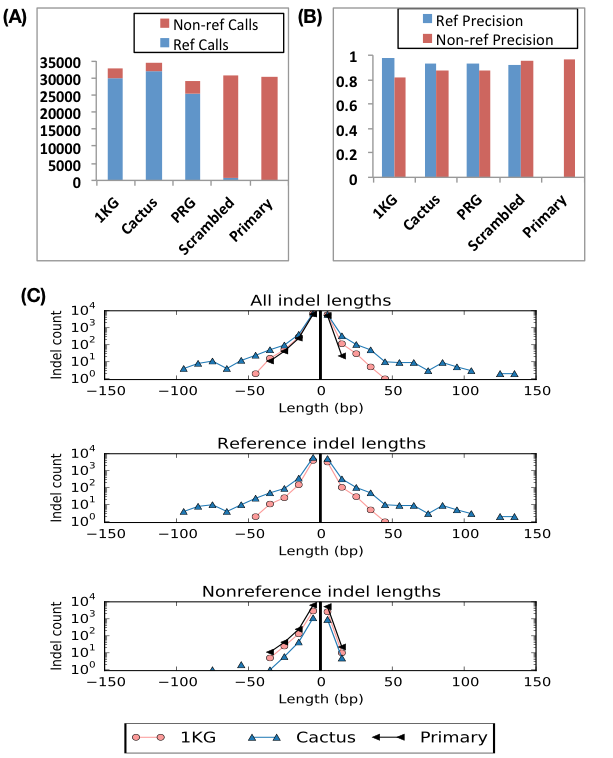
\includegraphics[width=2in]{figures/04_bakeoff/figure05.png}
\caption[Reference versus non-reference calls]{Reference versus Non-reference Calls. (A) Total number of
reference and non-reference calls across all samples and regions. (B)
Precision of reference and non-reference calls. (C) Indel lengths of
reference and non-reference calls, where insertions and deletions are
represented by positive and negative lengths, respectively. In all cases
we ignore calls of GRCh38 reference alleles, as these numbers are
reported from GRCh38-based output VCFs.}
\label{fig:bakeoff:refnonref}
\end{FPfigure}

\subsection{Short Path Accuracy}

We sought to understand how complete and accurate the sequence graphs
studied were in their representation of common variants. To approximate
this, we measured the fraction of lightly error-pruned K-mer instances
(here K=20, see Online Methods) in a large subset of 1KG sequencing
reads that were present within each graph, calling this metric
\emph{K-mer recall} (see Online Methods). We observe (Fig. \ref{fig:bakeoff:shortpaths},
Supplementary Section 9, and Supplementary Fig. 14) that graphs built
from the largest libraries of variation contain the great majority of
such K-mer instances. For example the 1KG, PRG and Cactus graphs contain
an average across regions of 99\% of K-mer instances, while the primary
graph contains an average across regions of 97\%. Conversely, we asked
what fraction of 20-mer instances present in a graph were not present in
any 1KG read, calling this metric \emph{K-mer precision}. Strikingly, we
find that precision is greatly reduced in some graphs relative to
control. For example around 15\% (averaged across regions) of 20-mers
enumerated from 1KG graphs do not appear in any 1000 Genomes low
coverage read. We hypothesize that this is because the density of
variation is sufficient in such graphs to admit many paths implying
recombinations that are either absent or very rare in the population. To
attempt to raise precision, for the 1KG data we constructed graphs using
haplotype information to eliminate a substantial subset of unobserved
paths, creating the ``1KG Haplo 50'' graph (Supplementary Section 10).
This resulted in increased precision (by about 10 percentage points in
BRCA2) with only a small reduction in recall, as shown in Figure \ref{fig:bakeoff:shortpaths} and
Supplementary Figure 13. However, this comes at the cost of a
performance degradation in read mapping (Fig. \ref{fig:bakeoff:mapping}) and variant calling
(Supplementary Section 7). One possible explanation for the performance
reduction is that the necessary duplication (``unmerging'') of paths in
this procedure reduced the aligner's ability to unambiguously map reads.

\begin{figure}[htbp]
\centering
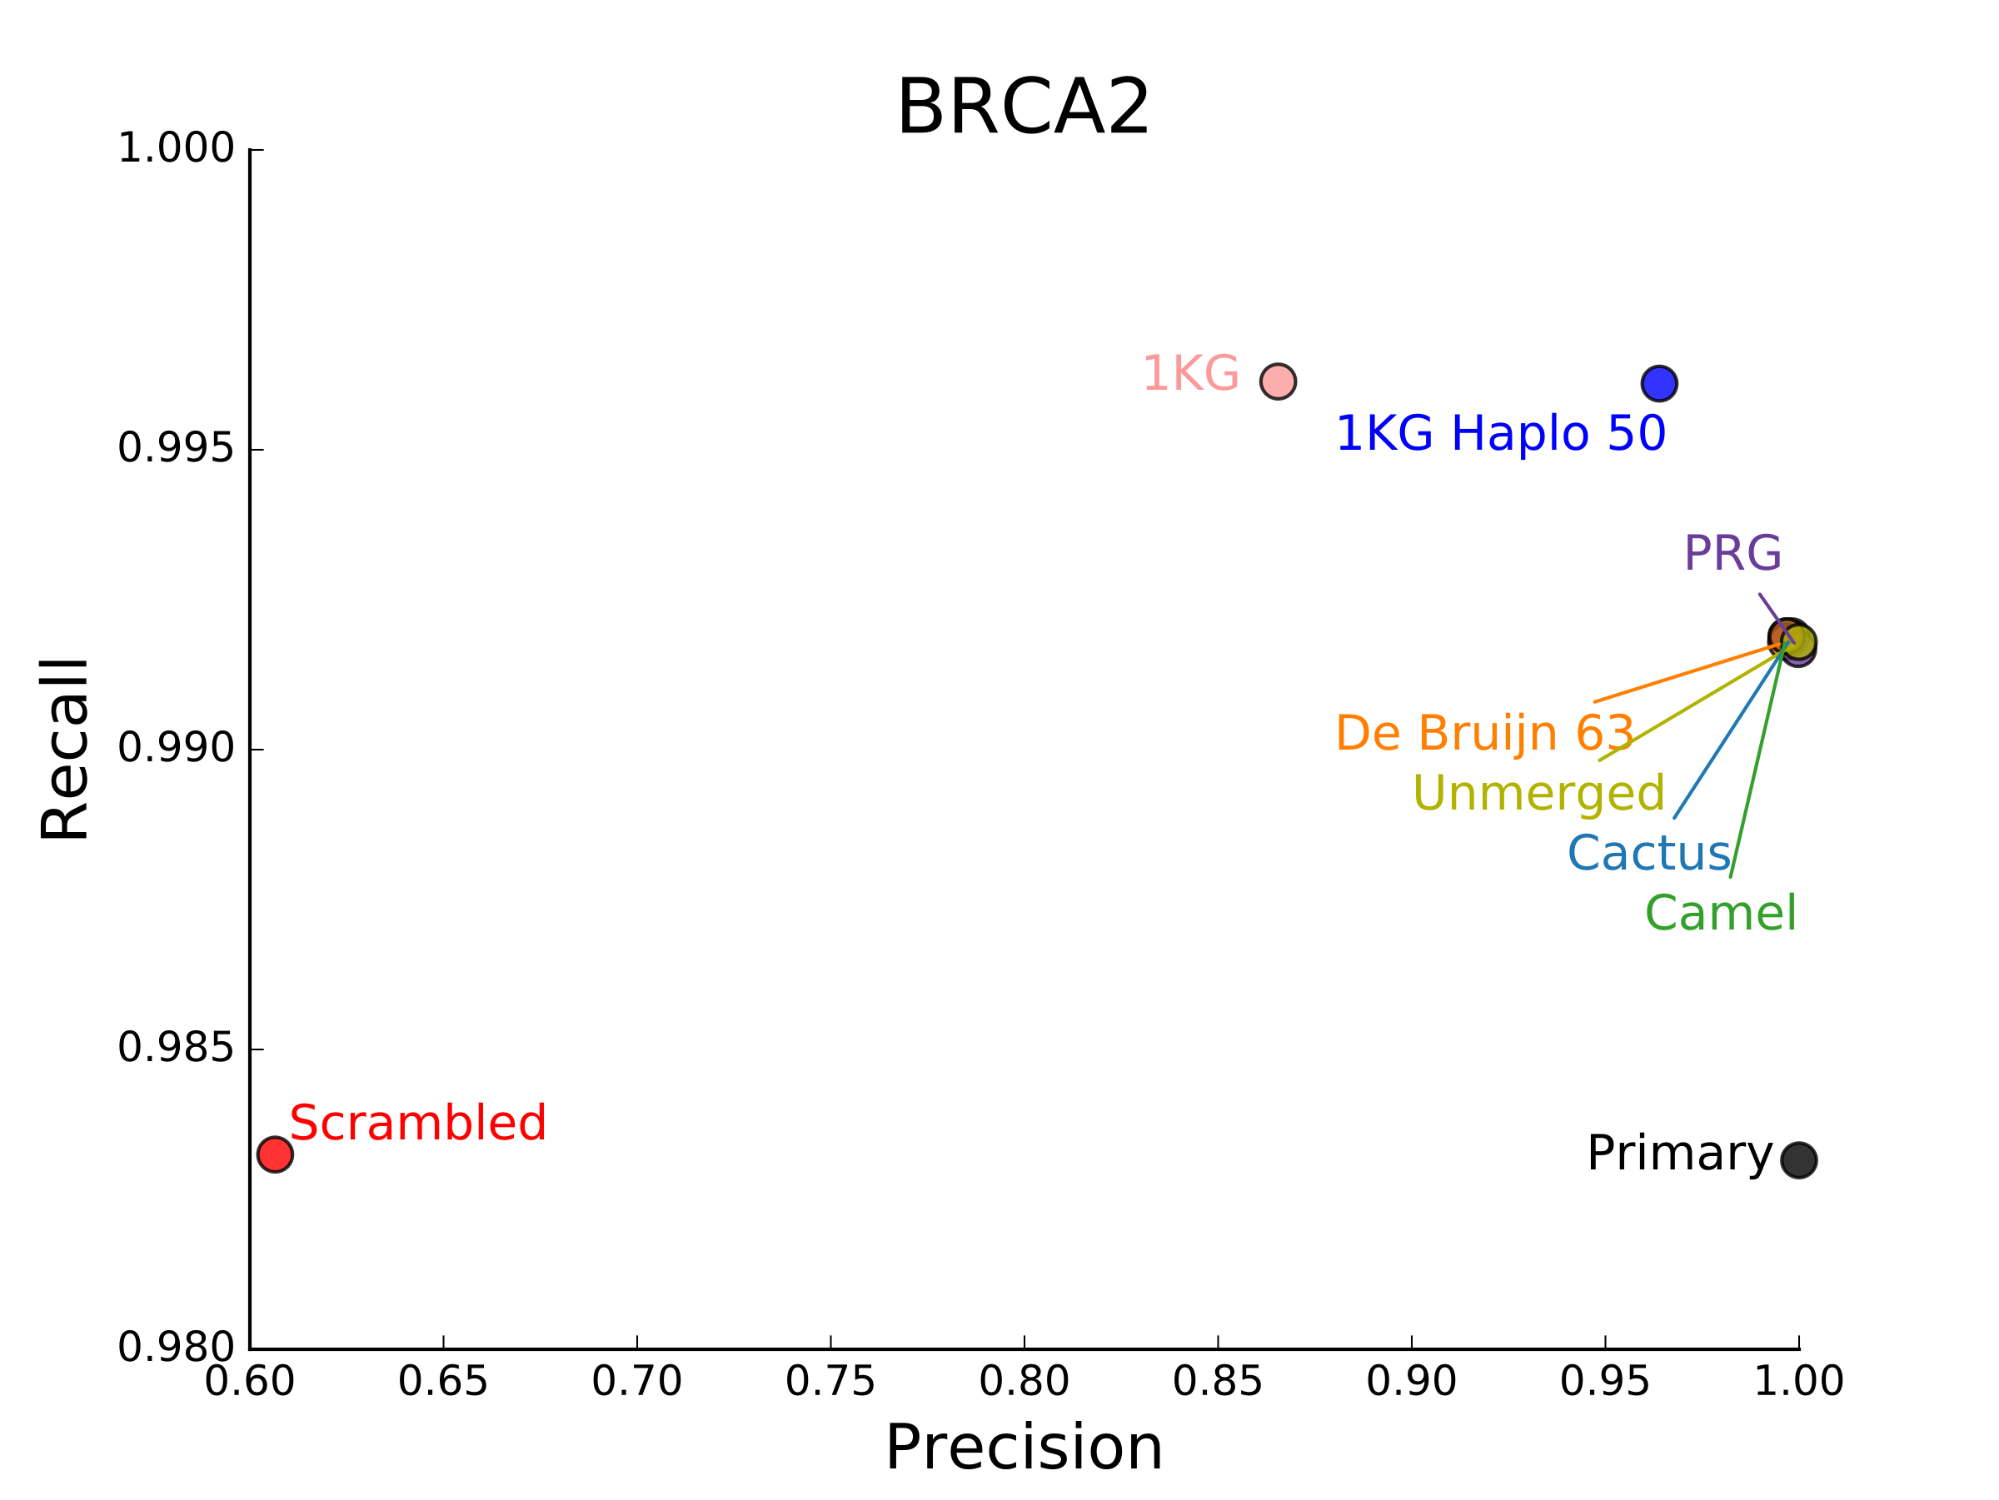
\includegraphics[width=0.5\textwidth]{figures/04_bakeoff/figure06_1.png}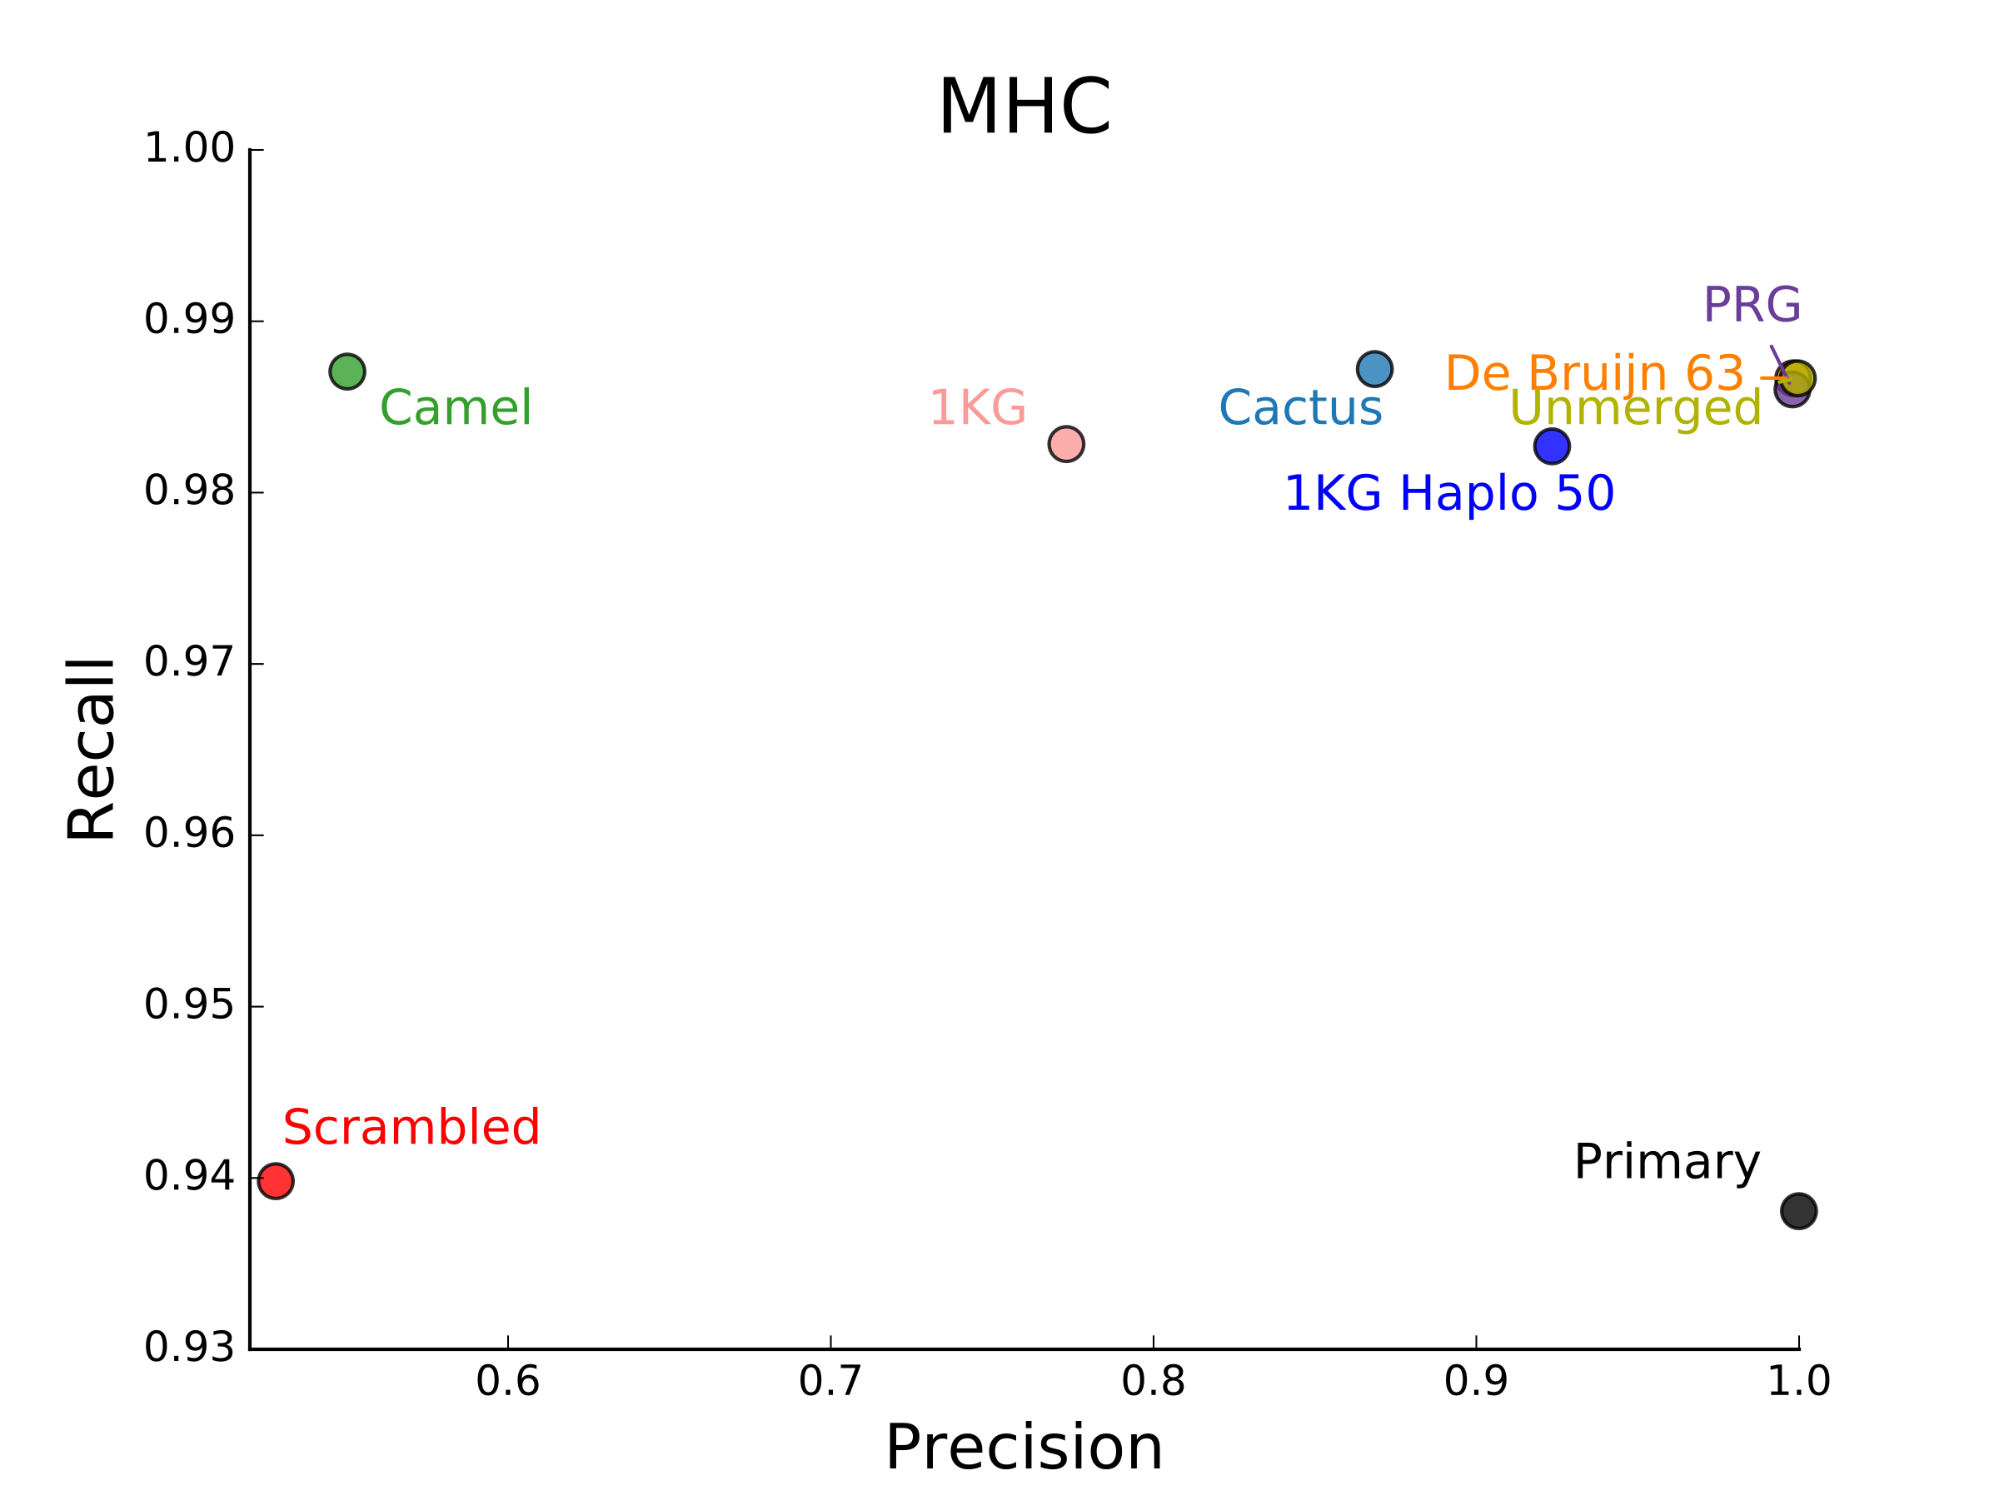
\includegraphics[width=0.5\textwidth]{figures/04_bakeoff/figure06_2.png}
\caption[Short path completeness and accuracy]{Short path completeness and accuracy. Assayed by comparing
20-mer instances.}
\label{fig:bakeoff:shortpaths}
\end{figure}

\subsection{Graph Character}

We found that even within each region the different submitted graphs
varied substantially in their performance on our evaluations of read
mapping and variant calling. They varied even more so with respect to
basic graph properties (Supplementary Section 11, Supplementary Tables
2-9). To quantify this variability we defined normalized graph metrics
for basic graph properties. \emph{Graph compression} is the length of
the primary reference sequence within the region divided by the sum of
the lengths of the nodes in the graph. It is a normalized measure of the
number of positions in the graph. The \emph{(base) degree} is the average
per-side degree of the graph in a bidirected graph representation with
single-base nodes, and is a measure of how much branching a graph
contains. The \emph{cut width} (Supplementary Table 10) is a measure of
apparent sequence rearrangement. Briefly, within a topologically sorted
graph, where all positions are ordered, cut width is the average over
all gaps between successive positions of the number of edges connecting
positions on the left side of the gap to positions on the right side of
the gap (Supplementary Section 12)\cite{haussler2017flow}. We see
wide variation in these measures across the graphs (Fig. \ref{fig:bakeoff:graphstats}).
Furthermore, across the different regions we find that there is an
inverse correlation (R=-0.674, p=0.00230) between cut width and variant
calling accuracy and a positive correlation (R=0.244, p=0.0268) between
compression and variant calling accuracy (Supplementary Fig. 15). The
base degree does not significantly correlate with variant calling
accuracy. These correlations suggest that uncompressed and highly
rearranged graphs do not work effectively with our current read mapping
and variant calling process.

\begin{FPfigure}
\centering
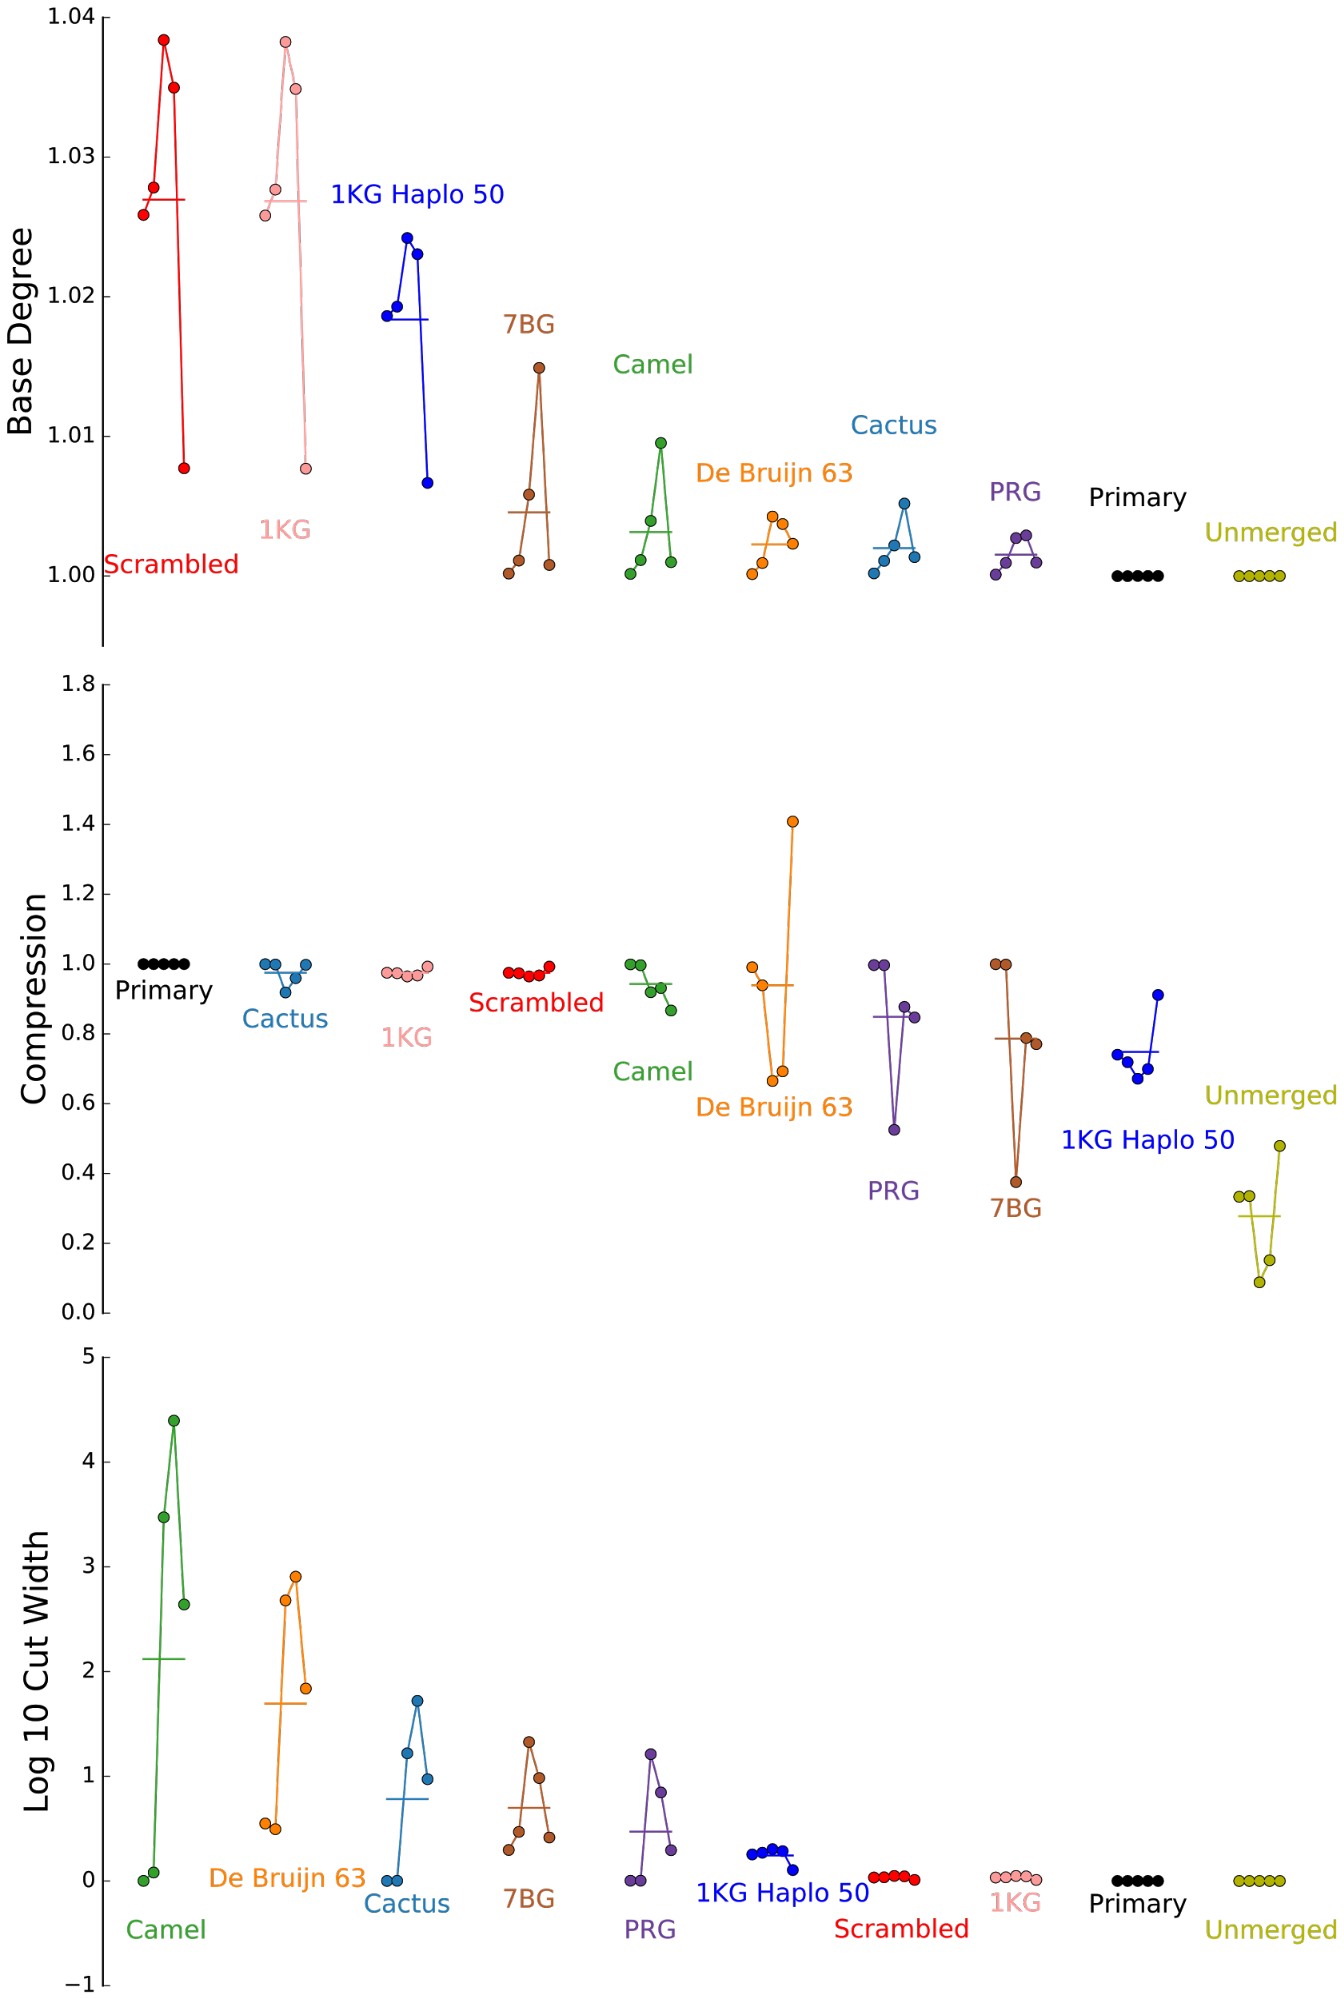
\includegraphics[width=0.9\textwidth]{figures/04_bakeoff/figure07.png}
\caption[Empirical graph statistics]{Empirical graph statistics. In each panel the result for each
region is shown by a dot, in the following order: BRCA1, BRCA2,
LRC\_KIR, MHC, and SMA.}
\label{fig:bakeoff:graphstats}
\end{FPfigure}

\section{Discussion}

Contemporary non-graphical variant calling procedures use different
algorithms for each class of variants: substitutions, small indels,
larger indels, balanced rearrangements, and so on. We have demonstrated
that variant calling on a sequence graph mostly obviates this
complexity, because being able to call the presence or absence of
elements within a sample graph is potentially sufficient for calling
known structural and point variation equally well. The simple, nascent
variant calling algorithm we tested produced variant calls that were
quite concordant with those from other state-of-the-art variant calling
pipelines, while unifying the calling of known SNPs and other known
structural variation. That individual tools slightly outperformed the
variant calling algorithm presented here in terms of individual variant
types, i.e.~snps and indels, is unsurprising given the relative maturity
and algorithmic sophistication of those tools. Importantly, many of the
submitted graphs showed improved variant calling performance over the
primary and scrambled graphs. The relative improvements come alongside a
large reduction in the number of non-reference calls. Furthermore,
reference calls were more accurate than non-reference calls, suggesting
that variant calling is indeed more accurate overall when the variants
themselves are contained within the graph. These results support the
notion that sequence graphs can transform variant calling by reducing it
to the simpler problem in which only rare variants, absent from the
graph, must be discovered de novo. It is possible to foresee cutting the
number of non-reference point variation calls from the millions, as in
standard genome wide pipelines today, to on the order of thousands (see
Supplementary Section 3).

During the course of the variant calling comparison, we developed an
appreciation for the shortcomings of relying solely on the Platinum
Genomes benchmark data as a truth set\cite{Eberle2016-zc}. A key concern
is that the Platinum Genomes calls were derived by means of a consensus
of contemporary methods, all of which use the existing linear reference
and BWA-MEM-based mappings. Additionally, compared to vg, the Platinum
Genomes dataset often uses different combinations of calls to ``spell''
the same haplotype. Moreover, it often omits calls necessary to spell a
haplotype because it is not confident in them. While the omitted calls
are in regions marked as low confidence, a variant normalizer cannot
normalize a call that is not there. To get around these problems and
potential biases we introduced a reference-free method for assessing
variation calls. This evaluation demonstrated good consistency with the
Platinum Genomes in terms of the relative ranking of the different
methods evaluated, and demonstrated clearly that the best graph methods
slightly outperform existing methods.

Supporting the observed improvements in variant calling, we demonstrate
that read mapping can be made both more comprehensive and less ambiguous
with sequence graphs. Increases in perfect mapping and reductions in
substitution and indel rates were broadly consistent with the effect we
would expect if the graphs were representing the majority of common
polymorphisms, leaving the residual read error rates to account for the
majority of alignment differences. In this sense read mappings were
demonstrated to be less locally ambiguous, with mismatches and edits
having a more clearly defined meaning. Furthermore, the fact that read
mappings were also less globally ambiguous (i.e.~more certain in their
overall placement within the genome) is perhaps surprising. We thought
at the outset that using detailed graphs would have the drawback of
increasing the number of times a read maps to two or more places by
increasing the sheer number of mapping possibilities. However, we found
that the opposite is true - the addition of known polymorphisms to the
graph allows reads to better distinguish their true mapping location
from secondary, paralogous locations. Scaled genome-wide, these
improvements could help canonicalize mapping to the vast majority of
variation, which will become especially important as genome variants are
increasingly used in the clinic. The increases in perfect mapping could
also allow alignment to be made more efficient by allowing larger, more
stringent seeds or more aggressive ungapped matching. Our early work
with vg indicates that there is ample opportunity for improvement and
investigation of these novel approaches to the design of
high-performance mapping algorithms. We also collected some preliminary
data that suggests that the gains in mapping obtained by moving from the
existing reference to a graph like the 1KG graph are super-population
specific, suggesting that sequence graphs have the potential to reduce
the local ethnic bias inherent in a single reference genome.

By taking a community approach, we were able to sample a wide variety of
the contemporary software for building sequence graphs. It is apparent
that different methods produce dramatically different graphs, as
measured both by direct graph analysis and by practical performance as a
reference for common genomics tasks, suggesting that the field is just
in its formative stages. In trying to understand how ``complete'' and
``accurate'' graphs built with today's methods are at representing short
sequences present in the population, we encountered several surprises.
In particular, we found a large number of short non-biological paths
created within the highest degree graphs, such as the de Bruijn graphs,
parts of the 1KG graphs, and certain of the Seven Bridges graphs. We
tried modifying the 1KG graphs to reduce the number of false
recombination possibilities without much success. We may in the future
find that we can tolerate these short non-biological paths, or that
another approach is needed to eliminate them.

One alternative approach is to create uncompressed, lower-degree graphs
by duplicating variable regions to directly represent haplotypes, but it
is likely that, as demonstrated by the 1KG Haplo 50 and (at the logical
extreme) Unmerged graphs, the resulting long, equivalent sequence paths
would create too much multi-mapping ambiguity. Perhaps a better solution
may be the use of haplotype information embedded within the sequence
graph\cite{novak2016graph}, making it a \emph{variation graph}. This would
allow algorithms to map to a common graph coordinate system while
accounting for variants, read errors, and recombinations within the
mapping process itself. This approach would eliminate the need for
several inelegant heuristics used in contemporary linear-reference-based
analysis pipelines
\cite{1000_Genomes_Project_Consortium2012-gr,McKenna2010-bg}.

Sequence graphs can now be built from libraries of common variants, and
tools like vg, though still experimental, illustrate the huge potential
of the graph-based approach. There are a number of questions yet to be
tackled. How should duplications and repeats be represented? How can one
best map to a graph? How should short variants whose homologies are
unclear be parsed? How can graphs be used to enable a more comprehensive
taxonomy of variation? These questions all represent open avenues for
future research.

\section{Online Methods}

\subsection{Source Data}

Participants were provided with a data set consisting of five genomic
regions (BRCA1, BRCA2, LRC\_KIR, SMA, and MHC) to use in the creation of
their graphs. The data set came in the form of a ``reference'' sequence
and one or more ``alternate'' sequences for each region. For the
LRC\_KIR, SMA, and MHC regions, those alternate sequences were the alt
loci present in GRCh38.p2 for the regions of the same names in the
assembly, with the reference being the portion of the corresponding
chromosome encompassing the chromosomal coordinates for all of the alts.
The reference regions for BRCA1 (ID 672) and BRCA2 (ID 675) were
downloaded from Entrez Direct, while alternate sequences were the
annotated genes from the CHM1 hyatidiform mole assembly, and the LRG
sequences for those genes
\cite{Kans2016-ca,MacArthur2014-dh,Chaisson2015-wd}. Some participants
used additional source data in constructing their graphs.

\subsection{Graph Format}

All graphs were generated in or converted into an SQL text format for
submission. The graphs were then loaded into databases compatible with
the GA4GH Graph Reference Server, and servers for the graphs were hosted
on a Microsoft Azure cloud instance. Individual evaluation tools hit
against these API endpoints. For read alignment and variant calling
purposes, graphs were downloaded from the servers using the sg2vg
converter tool, written for this project, and stored in .vg graph
format. This on-disk format could be efficiently indexed for read
alignment---a function that the GA4GH server did not support---and so
was preferred for evaluations dependent on read alignment. The graphs
themselves were created using a variety of methodologies and approaches,
detailed in Supplementary Section 10.

\subsection{Alignment Target Quality}

The submitted graphs were used to align reads from 2,691 low-coverage
samples from the 1000 Genomes project, which had been aligned to GRCh38
with BWA-MEM \cite{Li2009-tj}. Alignments to the primary reference and,
where available, the GRCh38 alt loci for a region were downloaded using
Samtools \cite{Li2009-je}. The process took advantage of the tool's
ability to subset indexed files over FTP in order to obtain just reads
mapped within the region \cite{Li2009-je}. Next, the alignments were
converted into reads, yielding the relevant reads for that sample and
region. Unpaired reads in the downloaded set were discarded. An attempt
was made to correct for a known data corruption bug in the version of
BWA-MEM used to produce the alignments, by taking the sequences given
for alignments to the primary reference over the sequences given for the
same read aligned to an alt, where available (Heng Li, personal
communication). Input graphs were downloaded from the reference servers
using the sg2vg program. They were then broken into nodes of no more
than 100 bases each and re-numbered according to a heuristic extension
of topological sort to cyclic graphs. Graphs were indexed and alignment
was performed with the vg program, using a K-mer size of 16 and an
edge-crossing limit of 3 for the GCSA2 index. The portion of reads
mapping uniquely was calculated. To qualify as uniquely mapped, a read
had to have a primary mapping with 0.95 matches per alignment column or
fewer. Additionally, qualifying reads had to have either no secondary
mapping or a secondary mapping having fewer than 0.85 matches per
column. The denominator for the portion mapping uniquely was the number
of reads having either a secondary mapping distinct from the read's
primary mapping or no secondary mapping at all (see Supplementary
Section 3). The portion of reads mapping perfectly was defined as the
portion having 1 match per alignment column. The substitution rate was
defined as the portion of bases in length-conserving replacements out of
all substituted or matched bases. Bases matched or substituted against N
characters in the reference graph were ignored. The indel rate was
defined as indel count divided by substituted and matched bases. Bases
matched or substituted against reference Ns were ignored, as were indels
that constituted softclips.

\subsection{Platinum Genomes Variant Calling Evaluation}

A graph variant calling pipeline based on the Samtools pileup method was
implemented in vg and run independently on three 50x coverage samples
from Platinum Genomes (NA12877-9). First, the reads were mapped to each
graph as described above. The alignments were then filtered to remove
secondary mappings, as well as mappings with mapping quality score less
than 15, mappings that had been promoted to primary over another
properly paired mapping of greater single-end score, and mappings with
soft-clipped or ambiguous ends (more details in Supplementary Section
7). A pileup of aligned read bases was then constructed for each
position and edge in the graph ignoring bases with read quality score
less than 10. The SNPs, insertions, and deletions implied by the two
most supported non-reference entries in each pileup were then added into
the graph to create an ``augmented'' graph. Sites in the augmented graph
were computed using the ultrabubbles
algorithm\cite{paten2017superbubbles}. For each site, the two
non-reference paths with the most read support were greedily chosen
using a breadth-first search. A path's read support was defined here as
the minimum pileup support of any node or edge it contains; each node's
support was calculated as the average support across the node's bases.
Finally, given the reference path and these two alternate paths for each
site, a genotype was computed using a thresholding heuristic based on
the ratios of the paths' pileup supports. Alternate alleles were called
as heterozygous if they had at least three times as much read support as
the reference (or six times for a homozygous alt call). The genotypes
were written directly to VCF. The variants were normalized by using
vt\cite{Tan2015-fv} to flatten multibase alts that contain reference
calls. Calls for both NA12877 and NA12878 were compared against their
respective Platinum Genomes truth set VCFs; these were the only samples
with truth VCFs available. Precision and recall against the truth set
were assessed with vcfeval\cite{Cleary2015-oy}. True and false positives
and negatives returned from this tool were classified as SNPs and indels
using bcftools, and clipped into the Platinum Genomes confident regions.
Precision, recall and F1-scores were then computed for each possible
quality threshold in the VCF. For the vg call results, minimum read
support (AD field in VCF genotype) across called alleles was used as a
proxy for quality. Aggregate results across samples and regions were
computed by pooling the vcfeval results together. The precision-recall
curves (Fig. \ref{fig:bakeoff:callingeval} (C) and (D)) were drawn by filtering the VCF files by all
values of variant quality and displaying only those within distance 0.1
of the maximum F1-score. The points shown in Figure \ref{fig:bakeoff:callingeval} (A) were chosen to
correspond to the quality threshold yielding the maximum F1-score.

\subsection{Reference-Free Evaluation}

A ``synthetic diploid'' genome was conceptualized by combining data from
two haploid samples, CHM1 and CHM13\cite{Steinberg2014-pu}. For each
sample, GRCh38-aligned low-coverage Illumina reads and relatively
complete PacBio-derived assemblies were obtained. The CHM1 and CHM13
reads were obtained by combining both runs from NCBI SRA SRX1391727 and
SRX1082031, respectively, and mapping to GRCh38 using
BWA-MEM\cite{Li2009-tj}. The CHM1 assembly used was GenBank accession
number GCA\_001297185.1, while the CHM13 assembly was GCA\_000983455.2.
For each region, a pooled collection of the relevant Illumina reads
across both CHM1 and CHM13 was created. Next, the reads were subsampled
for balanced coverage between the two haploid genomes as would be
expected in a real diploid sample. For each submitted graph under tests,
the reads were aligned using vg, and the vg variant caller was used to
produce variant calls. The resulting VCF for each graph construction
method and region combination was turned into a new ``sample graph'' to
which the relevant portions of the PacBio assemblies were aligned.
Treating the aligned assembly fragments as the truth, the precision and
recall of each sample graph were measured as a function of which
original submitted graph it was derived from.

Assembly fragments used for evaluation were selected by alignment of the
primary reference sequences for the regions against the CHM1 and CHM13
assemblies using BLAT version 36x2~\cite{Kent2002-wo}. Aligned regions
in the assembly covering more than either 50\% of an assembly contig or
50\% of a region, with more than 98\% identity, were extracted from the
assembly and used for realignment. The SMA region was excluded from the
evaluation due to patchy, overlapping coverage of the region in the two
assemblies. Additionally, the first 87,796 bases of the LRC\_KIR region
were excluded from the sample graphs and the aligned truth set contigs
due to an apparent lack of representation in the CHM13 assembly.

\subsection{Assessing Graph Completeness}

Reads aligning to the test regions were obtained from 2,691 low-coverage
samples in the 1000 Genomes Project, and each sample's reads were used
to generate a collection of K-mers (K=20) using Jellyfish
\cite{Marcais2011-ck,1000_Genomes_Project_Consortium2015-mp}. These were
compared against the collection of K-mers in each graph as enumerated by
vg with an edge-crossing limit of 7. In order to account for K-mer
frequencies, duplicate K-mers were \emph{not} ignored. K-mers containing
N characters were ignored in both collections, and K-mers only observed
once in their sample were ignored in the 1000 Genomes-derived K-mer
collection. This latter filter was intended to remove the large majority
of erroneous K-mers: we expect errors to be Poisson-distributed one-off
events while real variants are likely to recur within a sample. Recall,
defined as the portion of all read-derived K-mers present among the
graph-derived K-mers, and precision, defined as the converse, were
computed for each graph.

\subsection{URLs}

\begin{itemize}
\item[] VG, \href{https://github.com/vgteam/vg}{https://github.com/vgteam/vg}.

\item[] Patches to VG,
\href{https://github.com/adamnovak/vg/tree/graph-bakeoff}{https://github.com/adamnovak/vg/tree/graph-bakeoff}.

\item[] GA4GH to VG Importer,
\href{https://github.com/glennhickey/sg2vg}{https://github.com/glennhickey/sg2vg}.

\item[] VG to GA4GH Exporter,
\href{https://github.com/glennhickey/vg2sg}{https://github.com/glennhickey/vg2sg}.

\item[] GA4GH Graph Schemas,
\href{https://github.com/ga4gh/schemas/tree/refVar-graph-unary}{https://github.com/ga4gh/schemas/tree/refVar-graph-unary}.

\item[] GA4GH Graph Server,
\href{https://github.com/ga4gh/server/tree/graph}{https://github.com/ga4gh/server/tree/graph}.

\item[] Graph evaluation software,
\href{https://github.com/BD2KGenomics/hgvm-graph-bakeoff-evaluations}{https://github.com/BD2KGenomics/hgvm-graph-bakeoff-evaluations}.

\item[] FASTG,
\href{http://fastg.sourceforge.net/}{http://fastg.sourceforge.net/}.

\item[] Illumina Platinum Genomes,
\href{http://www.illumina.com/platinumgenomes/}{http://www.illumina.com/platinumgenomes/}.

\item[] Jellyfish,
\href{http://www.cbcb.umd.edu/software/jellyfish/}{http://www.cbcb.umd.edu/software/jellyfish/}.

\item[] Platypus,
\href{http://www.well.ox.ac.uk/platypus}{http://www.well.ox.ac.uk/platypus}.

\item[] Freebayes,
\href{https://github.com/ekg/freebayes}{https://github.com/ekg/freebayes}.

\item[] Samtools, \href{http://www.htslib.org/}{http://www.htslib.org/}.

\item[] VCFeval,
\href{https://github.com/RealTimeGenomics/rtg-tools}{https://github.com/RealTimeGenomics/rtg-tools}.
\end{itemize}

\subsection{Software Versions and Commit Hashes}

\begin{itemize}
\item[] VG, 158d542497445b532b0e9e40223f5023ee6b52dd.

\item[] GA4GH to VG Importer, 468026ad70f0425af1959b287ffcaac91b8a9deb.

\item[] VG to GA4GH Exporter, 4efde8e64a8bd113a0e83685628bbaf0cbc2be3f.

\item[] GA4GH Graph Schemas, ea58ac46dad84be67c500e517ff2fb05a43a187a.

\item[] GA4GH Graph Server, c6daebca4c69a4ff4d9d56cfdf587556f2ce1116.

\item[] Graph evaluation software, 52b0537713629471f6ea97ccf552d6727c630f3d.

\item[] Freebayes, 9e983667d47f6b5dcbb90070da8de69714038f46.

\item[] Samtools, version 1.3.1.
\end{itemize}

\subsection{Acknowledgments}

This work would not have been possible without the generous support of
the National Human Genome Research Institute (1U54HG007990 {[}BD2K{]} to
B.P. and D.H., 5U41HG007234 {[}GENCODE{]} to B.P.); the W. M. Keck
Foundation (DT06172015 to B.P. and D.H.); the Wellcome Trust
(100956/Z/13/Z to G.M.); the Simons Foundation (SFLIFE\# 351901 to B.P.
and D.H.); the ARCS Foundation (2014-15 ARCS fellowship to A.M.N.) and
Edward Schulak (Edward Schulak Fellowship in Genomics to A.M.N.).

\subsection{Author Contributions}

A.M.N. contributed the Camel graphs, wrote read mapping and variant
calling code for vg, ran the read mapping and reference-free
evaluations, and contributed extensively to the organization of the
manuscript. G.H. contributed the Cactus, 1KG, 1KG Haplo 50, Primary, and
Scrambled graphs, and performed the variant calling evaluation. E.G.
contributed the bulk of the vg tool. S.B. contributed the analysis of
graph statistics. A.C., S.G., N.O., and A.W.Z. contributed the Curoverse
graphs, with A.W.Z. supervising. A.D., J.K., supervised by G.MV.,
contributed the PRG graphs. J.E. contributed alignment code to the vg
tool. M.A.S.E. contributed advice and corrections to the manuscript.
A.K. contributed the De Bruijn 63 graphs. S.K. contributed code to the
GA4GH graph server and contributed extensive organizational support.
D.K. and G.R. contributed the SBG graphs. H.L. contributed experimental
design support for the read mapping evaluation, and advice on the
manuscript. M.L. worked on scaling up the variant calling pipeline to
whole genomes. K.M. contributed a set of graphs for the chromosome X
centromere. M.S-O. contributed code to the GA4GH graph server and
managed the graph data import pipeline for this work. R.D. contributed
to the design of the GA4GH graph server interface and schemas, and
supervised other authors. G.M., D.H., R.D. and B.P. contributed to the
design of the project and supervised authors. B.P. and organized the
project directly, and wrote extensive portions of the manuscript. All
authors edited the manuscript.

